‎\documentclass[a4paper,12pt]{book}‎
\usepackage{graphicx}
\usepackage{graphics}
\usepackage{epsfig}
\begin{document}
\begin{flushright}
INTRODUCTION
\hspace{6mm}
7
\end{flushright} 
\vspace{3mm}
creative minds will develop new tools uniquely designed for producing both knowledge and wisdom in the virtual context. Thus, e-research is concerned both with the application and adoption of tools from the real world and the invention, refinement, and calibration of a new genre of tools.

We are convinced that a networked society is not a fad and that we are at the beginning of a new era in human collective activity. This era is not marked by elimination of the value or unique functionality of face-to-face and place-bound interaction. Rather, it represents the growth of parallel and alternative forms of many types of human interaction and discourse. These parallel forms are not inherently better, nor worse, than pre-Net forms of interaction and education. However, network-enhanced interaction better fulfills some human needs at certain points in time by providing access, convenience, utility, speed, and cost-effectiveness. These attributes result in the eager exploration of cyberspace by many citizens, thereby creating a new human context that selectively, and individually, forms a terged environment of networked and face-to-face environments. We know little of this merged context-either at a macro level or at the individual interaction level. Thus, e-research is critically important in providing a means to first understand and then to create a networked social and economic context that assists individual human beings and their collective organizations to live productively, joyfully, and securely on our planet.
\vspace{3mm}
\hspace{-2.5cm}
\textbf{SCOPE OF e-RESEARCH}
\vspace{2mm}
As we researched this book, it became apparent that the network was becoming an integral component of many activities that had been undertaken previously using nonnetworked tools. It also became obvious that new forms of behavior and community were being established in which the existence and support of the network were necessary for the behavior to exist. Thus, the scope and extent of e-research is expanding at unprecedented levels. What we needed was a conceptual rubric to help us differentiate those forms of behavior and research activities that we were to examine in this book from those that we were to leave to other authors. Table 1.1 may be useful for the reader in understanding where this book fits in the larger arena of research and network writings. The shaded cells are the focus of this look-activities in the unshaded cells are adequately covered in earlier, more traditional research and methods texts. Table 1.1 illustrates that e-research works at two quite distinct levels: first as a new medium to undertake research tisks that were previously done using alternate media or without mediated tools at all and second as a tool that allows us to investigate activity that itself would not be possible without the Net.
\vspace{9mm}
\begin{flushleft}
\hspace{-20mm}
8
\hspace{6mm}
CHAPTER ONE
\end{flushleft} 
\vspace{4mm}

\vspace{2mm}
\hspace{-2.5cm}
\textbf{RESEARCH ATTRIBUTES OF e-RESEARCHl}
\vspace{5mm}

Studying the applications and communities that have formed in virtual space is a researchers' dream world due to the data collection that is often integral and automatically gathered during online activity. The inajor activity of many communities is

\vspace{5mm}
\hspace{-2.5cm}
\textbf{TABLE 1.1   \  Scope of e-Research-Possible Research Activities.}
\vspace{1mm}
\begin{figure}[tbh]
\begin{center}
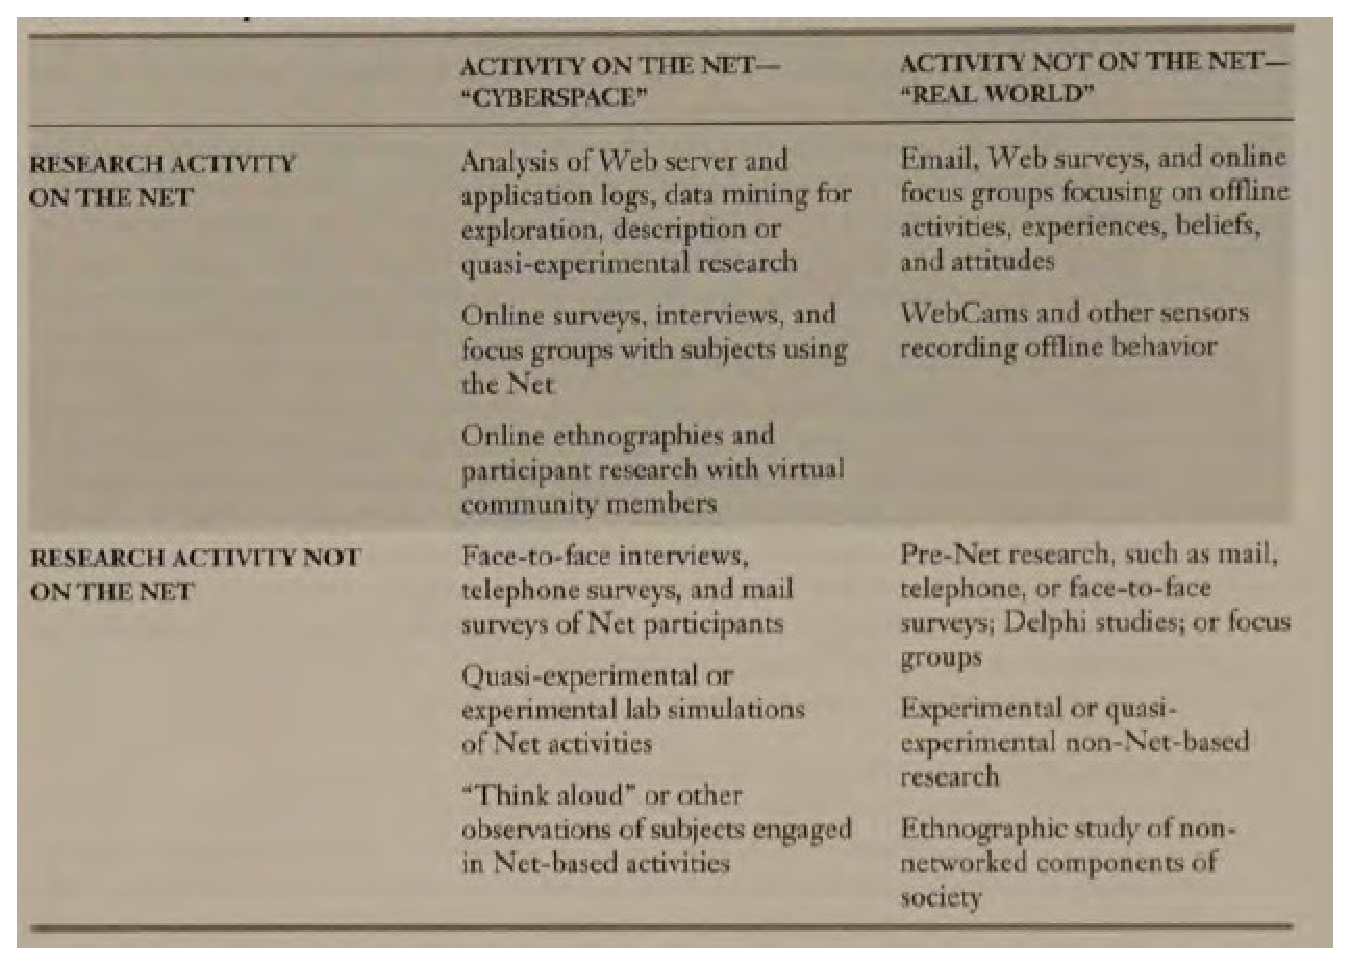
\includegraphics[width=11cm]{jadval.eps}
\label{fig_name}
\end{center}
\end{figure}
\hspace{-2.5cm}
\vspace{2mm}
verbal discourse and the transcript of this interaction is routinely captured and stored on the Net as text files. These files can readily be imported into text analysis tools, thus eliminating cost, time, and transcription. Second, the Net is renowned for the continuous tracking of most types of online activity, such as the sequence of participant activities at a site or the amount of use of an online resource. As such, it is capable of collecting valuable data that provide a unique window into human activity on the Net.
The Net also provides a unique 
context in which to study innovations in the social sciences and particularly in education. Modern learning theory stresses the value of muluple perspectives, of working with peers on collaborative and cooperative tasks, of searching and constructing information artifacts, and of exploring and learning in multicultural communities. The Net provides new and cost-effective possibilities for each of 
\vspace{5mm}
\begin{flushright}
INTRODUCTION
\hspace{6mm}
9
\end{flushright} 
\vspace{2mm}
these contexts. Many of the techniques being developed for online learning are finding application in the classroom--and vice versa. As we learn the unique educational capacity of both online and real-time classrooms, we will design learning exercises and activities that maximize each environment.
\vspace{1mm}
\hspace{-2.5cm}
\textbf{QUALITIES OF THE e-RESEARCHER}
\vspace{2mm}
This book is designed to help researchers become proficient e-researchers. It does so, not by describing step-by-step details or how to operate Net-based software (there are many books and other learning resources that address this task). Neither is it a book focused on developing generic or specific research skills—again there are specialized texts dealing with all of the methods and tools of good research practice. Rather, this book focuses on describing and illustrating, in clear and simple language, the variety of ways in which researchers may use the Internet to enhance their professional practice. We also provide suggested activities and links to related Internet sites. This combination of conceptual overview of network programs, practices, and operating processes, coupled with suggestions for hands-on activity, is designed to quickly increase the readers' self-efficacy in regard to both the skills of research and the capacity to effectively use networked resources.

Figure 1.1 illustrates the e-research skills that exist at the intersection of networking skills and research skills. The processes on the right of the diagram detail the course of research in any domain. We do not believe the function of each component of the research process is fundamentally different in either e-research or traditional research. The Internet skills listed on the left of the model are the prerequisite skills and capacity needed to be a competent network user. The e-researcher needs to develop these skills and will do so in the process of undertaking and completing an e-research project. Like other complex skills, there is no single minimal level of competency needed, but increasing skills at all levels results in more effective and efficient
\begin{figure}[tbh]
\begin{center}
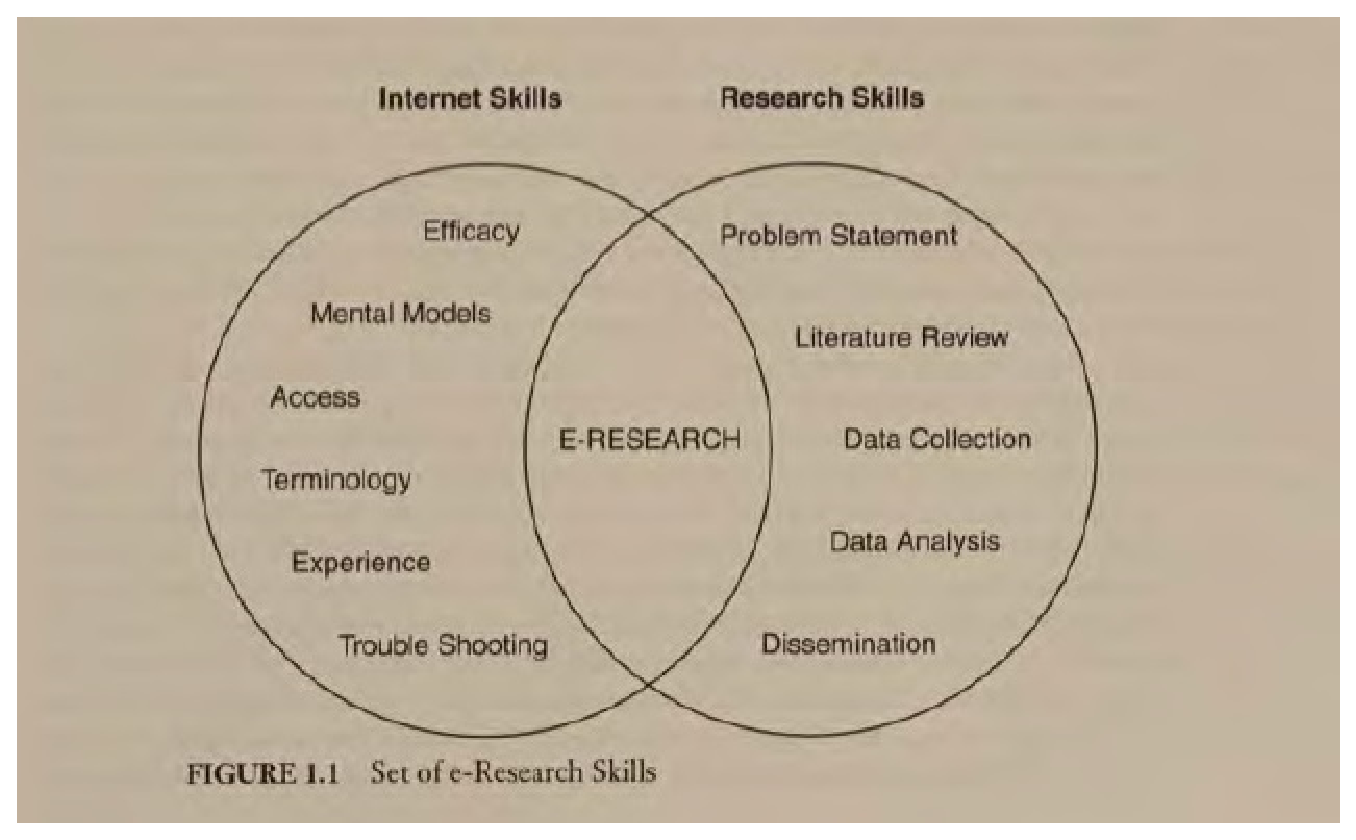
\includegraphics[width=8cm]{bv.eps}
\caption{Sct of e-Research Skills}
\label{fig_name}
\end{center}
\end{figure}
\vspace{2mm}





\end{document}
